\newcommand{\sysname}{Avalanche}

%We have fully implemented the proposed payment system.  In this section, we examine its throughput, scalability, and latency
%through a large scale deployment on Amazon AWS\@, and provide a comparison to known results
%from other systems.

\subsection{Setup}%\tronly{}{\vspace{-0.25em}}
% hardware setup
We conduct our experiments on Amazon EC2 by running from hundreds (125) to thousands (2000)
of virtual machine instances.  We use \texttt{c5.large} instances, each of
which simulates an individual node. AWS provides
bandwidth of up to 2 Gbps, though the {\sysname} protocol utilizes at most around 100 Mbps.

% the transaction specification
Our implementation supports two versions of transactions: one is the customized UTXO format,
while the other uses the code directly from Bitcoin 0.16. Both supported formats use secp256k1
crypto library from bitcoin and provide the same address format for wallets. All experiments
use the customized format except for the geo-replication, where results for both are given.

We simulate a constant flow of new transactions from users by creating
separate client processes, each of which maintains
separated wallets, generates transactions with new recipient addresses and
sends the requests to {\sysname} nodes.
%\textbf{[RVR: what is a ``full'' node? (fixed)]}
We use several such client
processes to max out the capacity of our system.  The number of recipients
for each transaction is tuned to achieve average transaction sizes of
around 250 bytes (1--2 inputs/outputs per transaction on average and a stable
UTXO size), the current average transaction size of Bitcoin. To utilize the
network efficiently, we batch up to 40 transactions during a query, but
maintain confidence values at individual transaction granularity.

% how do we measure throughput/latency
All reported metrics reflect end-to-end measurements taken from the perspective of all clients.
That is, clients examine the total number of confirmed
transactions per second for throughput, and, for each transaction,
subtract the initiation timestamp
from the confirmation timestamp for latency. Each throughput experiment is
repeated for 5 times and standard deviation is indicated in each figure.
%\tronly{Because we
%saturate the capacity of the system in all runs, some transactions
%will have much higher latency than most, we use the 1.5$\times$IQR rule
%commonly used to filter out outliers. Take the geo-replicated experiment as an example,
%$15.8\%$ data are the outliers having 6.63 second latency on average. They fall
%out of 1.5$\times$IQR (approximately $3\sigma$) range and are filtered out. There are very few outliers
%when the system is not saturated. All reported latencies (including maximum) are those not filtered.
%%\textbf{[RVR: how high are these outliers?  how many are there?  do they still happen if the system is not saturated? (fixed)]}
%}{}
As for security parameters, we pick $k = 10$, $\alpha = 0.8$, $\beta_1 = 11$, $\beta_2 = 150$, which yields an MTTF of \textasciitilde{}$10^{24}$ years.

\subsection{Throughput} %\tronly{}{\vspace{-0.5em}}

We first measure the throughput of the system by saturating it with
transactions and examining the rate at which transactions are confirmed in the
steady state.  For this experiment, we first run {\sysname} on 125 nodes
with 10 client processes, each of which maintains 400 outstanding transactions at
any given time.

As shown by the first group of bars in Figure~\ref{fig:eval-thr}, the system achieves
6851 transactions per second (tps) for a batch size of 20 and above 7002 tps for a batch size of 40.
Our system is saturated by a small batch size comparing to other blockchains with known performance:
Bitcoin batches several thousands of transactions per block, Algorand~\cite{GiladHMVZ17} uses 2--10 Mbyte blocks, i.e., 8.4--41.9K tx/batch and Conflux~\cite{confluxLLXLC18} uses 4 Mbyte blocks, i.e., 16.8K tx/batch. These systems are relatively slow in making a single decision, and thus require a very large batch (block) size for better performance. Achieving high throughput with small batch size implies low latency, as we will show later.

\begin{figure}[h]
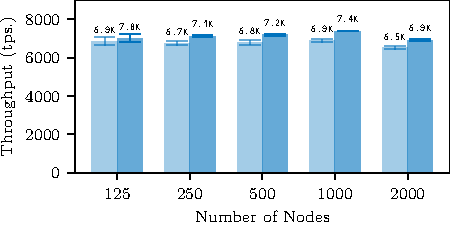
\includegraphics[width=\linewidth]{figures/thr-ava.pdf}
\captionof{figure}{Throughput vs. network size. Each pair of bars is produced with batch size of 20 and 40, from left to right.}
%    The slight degradation with doubled network sizes illustrates scalability.}
\label{fig:eval-thr}
\end{figure}

\begin{figure}
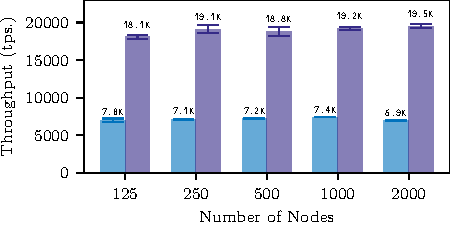
\includegraphics[width=\linewidth]{figures/thr-raw.pdf}
\captionof{figure}{Throughput for batch size of 40, with (left) and without (right) signature verification.}
\label{fig:eval-thr-raw}
\end{figure}

\subsection{Scalability}%\tronly{}{\vspace{-0.25em}}

To examine how the system scales in terms of the number of nodes
participating in {\sysname} consensus, we run experiments with identical settings
and vary the number of nodes from 125 up to 2000.

Figure~\ref{fig:eval-thr} shows that overall throughput degrades about $1.34\%$ to 6909 tps when the network grows by a factor of 16 to $n = 2000$.
This degradation is minor compared to the growth of the network size.
Note that the x-axis is logarithmic.
% , and thus throughput degradation is negligible.

Avalanche acquires its scalability from three sources: first,
maintaining a partial order that captures only the spending relations
allows for more concurrency than a classical BFT replicated
log that linearizes all transactions; second, the lack of a leader naturally avoids bottlenecks;
finally, the number of messages each node has to handle per decision is $O(k)$ and does not grow as the network scales up.
% Another way to view this is that {\sysname} implicitly performs similar to sharding with
% the help of the DAG, in that multiple nodes can work on different parts of the
% central data structure concurrently.
%{\sysname} trades off total order for a scalable system.

%(Figure 4: x-axis is the number of client processes, y-axis is the averaged latency)

%\tronly{{}
\subsection{Cryptography Bottleneck}%\tronly{}{\vspace{-0.25em}}

We next examine where bottlenecks lie in our current implementation.
The purple bar on the right of each group in Figure~\ref{fig:eval-thr-raw} shows the throughput of Avalanche with signature verification
disabled. Throughputs get approximately 2.6x higher, compared to the blue bar on the left.
This reveals that cryptographic verification overhead is the current bottleneck of our system implementation.
This bottleneck can be addressed by offloading
transaction verification to a GPU\@. Even without such optimization,
7K tps is far in excess of extant blockchains.
%}{}

\subsection{Latency}%\tronly{}{\vspace{-0.25em}}

\begin{figure}
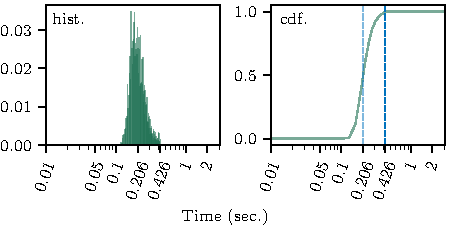
\includegraphics[width=\linewidth]{figures/lat.pdf}
\captionof{figure}{Transaction latency distribution for $n = 2000$. The x-axis
    is the transaction latency in log-scaled seconds, while the
    y-axis is the portion of transactions that fall into the confirmation
    time (normalized to $1$).  Histogram of all transaction latencies for a client is shown on the left with $100$ bins,
    while its CDF is on the right.}
\label{fig:eval-lat1}
\end{figure}

The latency of a transaction is the time spent from the moment of its
submission until it is confirmed as accepted.
%\textbf{[RVR: this is not quite clear to me.  Where is finality defined? (fixed)  I only see the isAccepted() predicate that checks finality, but I assume finality, whatever it is, is achieved before a client learns about it.]}
Figure~\ref{fig:eval-lat1} tallies
the latency distribution histogram using the same setup as for the throughput
measurements with 2000 nodes. The x-axis is the time in seconds while the y-axis
is the portion of transactions that are finalized within the corresponding
time period. This figure also outlines the Cumulative Distribution Function (CDF)
by accumulating the number of finalized transactions over time.


This experiment shows that most transactions are confirmed within approximately 0.3 seconds.
% The sharp transition that goes from nearly $0\%$ to $100\%$ shows that
The most common latencies are around 206 ms and variance is low,
indicating that nodes converge on the final value as a group around the same time.
The second vertical line shows the maximum latency we observe, which is around 0.4 seconds.
% (XXX: more on the distribution?)
%\textbf{[RVR: why use a log scale for the x-axis?  Is the transition really sharp? (yes) It doesn't look to me that way.  Is the 1.1 second maximum latency before or after removing outliers? (fixed) Is ``confirmation time'' the same as latency, and if so, why use different terms? (fixed)  The histogram is tiny... (yeah, because of cdf..)]}

Figure~\ref{fig:eval-lat2} shows
transaction latencies for different numbers of nodes.
The horizontal edges of boxes represent minimum,
first quartile, median, third quartile and maximum latency respectively, from
bottom to top.  Crucially, the experimental data show that median latency is more-or-less
independent of network size.
%\textbf{[RVR: the x-axis *should* be a log scale here.  It looks like a log scale but it is linear. (fixed)]}

\begin{figure}[h]
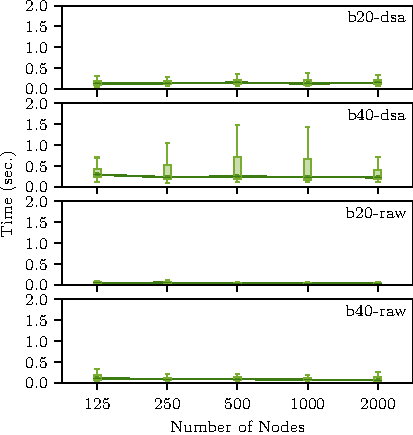
\includegraphics[width=\linewidth]{figures/lat2.pdf}
\captionof{figure}{Transaction latency vs. network size. ``b'' indicates batch size and ``raw'' is the run without signature verification.}
\label{fig:eval-lat2}
\end{figure}

\subsection{Misbehaving Clients}%\tronly{}{\vspace{-0.25em}}
\label{sec:evaluation-misbehaving}
\begin{figure}
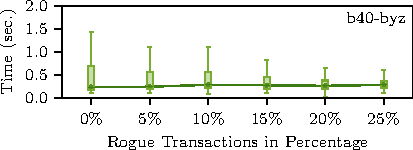
\includegraphics[width=\linewidth]{figures/lat3.pdf}
\captionof{figure}{Latency vs. ratio of rogue transactions.}
\label{fig:eval-lat3}
\end{figure}

We next examine how rogue transactions issued by misbehaving clients that
double spend unspent outputs can affect latency for virtuous
transactions created by honest clients. We adopt a strategy to
simulate misbehaving clients where a fraction (from $0\%$ to $25\%$) of the
pending transactions conflict with some existing ones.
%\textbf{[RVR: this is confusing, but maybe I should reread Section 2.  It used to be the case that it was impossible to create transactions that conflict with virtuous ones. (they double spend their own unspent outputs)]}
The client processes
achieve this by designating some double spending transaction flows among all
simulated pending transactions and sending the conflicting transactions to
different nodes. We use the same setup with $n = 1000$ as in the previous
experiments, and only measure throughput and latency of confirmed transactions.

{\sysname}'s latency is only slightly affected by misbehaving clients, as shown
in Figure~\ref{fig:eval-lat3}. Surprisingly, maximum latencies drop slightly when
the percentage of rogue transactions increases.  This behavior occurs
because, with the introduction of rogue transactions, the overall
\emph{effective} throughput is reduced and thus alleviates system load.
%\tronly{
This is confirmed by
Figure~\ref{fig:eval-thr2}, which shows that throughput (of virtuous transactions) decreases with the ratio of rogue transactions.
Further, the reduction in throughput appears proportional to the number of misbehaving clients,
that is, there is no leverage provided to the attackers.
%}{
%This is confirmed by throughput decreases with the ratio of rogue transactions.
%Further, the reduction in throughput appears proportional to the number of misbehaving clients,
%that is, there is no leverage provided to the attackers.
%}
%(XXX: is this universally true, or just for this attacker? Is this the strongest attacker we can imagine?)

\begin{figure}
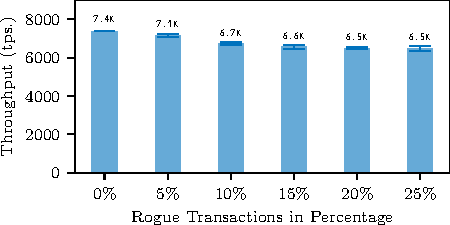
\includegraphics[width=\linewidth]{figures/thr-byz.pdf}
\captionof{figure}{Throughput vs. ratio of rogue transactions.}
\label{fig:eval-thr2}
\end{figure}

\subsection{Geo-replication}%\tronly{}{\vspace{-0.25em}}

\begin{figure}
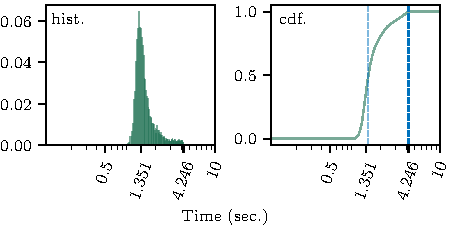
\includegraphics[width=\linewidth]{figures/lat4.pdf}
\captionof{figure}{Latency histogram/CDF for $n = 2000$ in 20 cities.}
\label{fig:eval-lat4}
\end{figure}

Next experiment shows the system in an emulated geo-replicated scenario, patterned
after the same scenario in prior work~\cite{GiladHMVZ17}.
We selected 20 major cities that appear to be near substantial numbers of reachable
Bitcoin nodes, according to~\cite{bitnodes2018}. The cities cover North America,
Europe, West Asia, East Asia, Oceania, and also cover the top 10 countries with the
highest number of reachable nodes. We use the latency and jitter matrix crawled
from~\cite{wondernetworkping2018} and emulate network packet latency in the Linux kernel using
\texttt{tc} and \texttt{netem}. 2000 nodes are distributed evenly to each
city, with no additional network latency emulated between nodes within the same city.
Like Algorand's evaluation, we also cap our bandwidth per process to 20 Mbps
to simulate internet-scale settings where there are many commodity network links.
We assign a client process to each city, maintaining 400 outstanding transactions per city
at any moment.

In this scenario, Avalanche achieves an average throughput of 3401 tps, with a standard deviation of 39 tps.
As shown in Figure~\ref{fig:eval-lat4}, the median transaction latency
is 1.35 seconds, with a maximum latency of 4.25 seconds. We also support native Bitcoin code
for transactions; in this case, the throughput is 3530 tps, with $\sigma = 92$ tps.


\subsection{Comparison to Other Systems}%\tronly{}{\vspace{-0.25em}}
Though there are seemingly abundant blockchain or cryptocurrency protocols,
most of them only present a sketch of their protocols and do not offer practical implementation or evaluation results.
Moreover, among those who do provide results, most are not evaluated in realistic, large-scale (hundreds to thousands of full nodes participating in consensus) settings.

Therefore, we choose Algorand and Conflux for our comparison. Algorand, Conflux, and Avalanche are all fundamentally different in their
% consensus principle and
design. Algorand's committee-scale consensus algorithm is quorum-based Byzantine agreement, and Conflux extends Nakamoto consensus by a DAG structure to facilitate higher throughput, while Avalanche belongs to a new protocol family based on metastability. Additionally, we use Bitcoin~\cite{nakamoto2008bitcoin} as a baseline.

Both Algorand and Avalanche evaluations use a decision network of size 2000 on EC2.
Our evaluation picked shared \texttt{c5.large} instances, while Algorand used \texttt{m4.2xlarge}\@.
These two platforms are very similar except for a slight CPU clock speed edge for \texttt{c5.large}, which goes largely unused because our process only consumes $30\%$ in these experiments.
The security parameters chosen in our experiments guarantee a safety violation
probability below $10^{-9}$ in the presence of $20\%$ Byzantine nodes, while
Algorand's evaluation guarantees a violation probability below $5 \times 10^{-9}$ with $20\%$ Byzantine nodes.

Neither Algorand nor Conflux evaluations take into account the overhead of cryptographic verification.
Their evaluations use blocks that carry megabytes of dummy data and present the throughput in MB/hour or GB/hour unit. So we use the average size of a Bitcoin transaction, 250 bytes, to derive their throughputs. In contrast, our experiments carry real transactions and fully take all cryptographic overhead into account.

The throughput is 3-7 tps for Bitcoin,
874 tps for Algorand (with 10 Mbyte blocks),
3355 tps for Conflux (in the paper it claims 3.84x Algorand's throughput under the same settings).

In contrast, {\sysname} achieves over 3400 tps
consistently on up to 2000 nodes without committee or proof-of-work.
As for latency, a transaction is confirmed after 10--60
minutes in Bitcoin, around 50 seconds in Algorand,
7.6--13.8 minutes in Conflux, and 1.35 seconds in {\sysname}.

Avalanche performs much better than Algorand in both throughput and latency
because Algorand uses a verifiable random function to elect committees, and
maintains a totally-ordered log while {\sysname} establishes only a partial
order. Although Algorand's leadership is anonymous and changes continuously,
it is still leader-based which could be the bottleneck for scalability, while
{\sysname} is leader-less.

Avalanche has similar throughput to Conflux, but its latency is 337--613x better.
Conflux also uses a DAG structure to amortize the cost for consensus and increase the throughput,
however, it is still rooted in Nakamoto consensus (PoW), making it unable to
have instant confirmation compared to Avalanche.

In a blockchain system, one can usually improve throughput at the cost of latency through batching. The real bottleneck of the performance is the number of decisions the system can make per second, and this is fundamentally limited by either Byzantine Agreement ($\mathrm{BA}^{*}$) in Algorand and Nakamoto consensus in Conflux.
